
\chapter{Semi-visible jets analysis (15/12/2017)}

Annapaola and her PhD student Giorgia have been developing the generation of samples and analysis of a dark matter search with semi-visible jets. Ben and I are planning to become involved in this, helping out where we can and hopefully providing some of the framework for my thesis. It is still early days and my first task is to use the code Giorgia has on GitHub to reproduce the sample generation in \PYTHIA. The short-term goal is to move the hard scattering aspect and matrix element calculations to \madgraph, and showering/hadronisation with \PYTHIA to produce samples that can be used in an analysis. MadGraph is better for simulating hard jets, whilst Pythia is better for softer objects.

The following are some slides Giorgia showed at the latest EXO workshop: \href{run:sec35/171201_GRauco_SVJ_InitialStudies.pdf}{171201\_GRauco\_SVJ\_InitialStudies.pdf}. She postulates that the dark sector consists of at least two "dark quarks" that interact via a new fundamental force. These dark quarks can couple to SM particles via a $Z'$ gauge boson that's leptophobic. The heavier, unstable dark sector particle is created in a collider via $pp \rightarrow Z' \rightarrow \chi_2 \bar{\chi}_2$. The $\chi_2$ then decays into the lighter, stable dark matter $\chi_1$ and jets. The dark matter is recorded as MET, whose direction is roughly collinear with the jets. The rest of the slides discuss the sample generation, event selections, and comparisons to the paper her work has been based off so far: Ref.~\cite{Cohen:2015toa}. Perhaps coincidentally, this is the same paper I read last year. I have a summary in Sec.~\ref{sec:svjoverview}.

A follow-up paper by the same authors was published in 2017: Ref.~\cite{Cohen:2017pzm}. This a longer, more-detailed description of the signatures and searches for semi-visible jets. They also include a GitHub repo to the input files needed to generate signal MC events in MadGraph and shower with Pythia: \url{https://github.com/smsharma/SemivisibleJets}. They were created with \textsc{FeynRules}, which can calculate Feynman rules and generate files for new models: \url{http://feynrules.irmp.ucl.ac.be/}.


\section{Summary of model}

% ADD MORE IN-DEPTH STUFF HERE: SU_d(2), QCD-LIKE DARK FORCE. DARK PARTICLES CHI_1 (DARK MATTER), CHI_2 (UNSTABLE), BOTH HAVE A DARK-QCD CHARGE, BUT NO QCD OR EM CHARGE. CHI_2 CAN DECAY EITHER INTO CHI_1 PAIR OR QUARK PAIR. ADD FEYNMAN DIAGRAM. ADD DIFFERENCES BETWEEN S- AND T-CHANNEL. DARK HADRONISATION USES "LUND STRING" FRAGMENTATION MODEL (REFERENCE~\cite{Andersson:1983ia}) LIKE REGULAR QCD.


\section{Current sample generation in \PYTHIA}

I forked Giorgia's repo at \url{https://github.com/grauco/SVJ_production} and set up a working directory on Soolin (\textbf{/storage/eb16003/Semi-visible\_jets/}). These consist of three bash scripts that create the Pythia config and batch submission scripts, and then use them to run the sample production on a cluster (where the Tier 3 machine at Zurich is only supported system, at the moment).

The script \textbf{set\_config.sh} sets up the environments and initialisation, taking care of CMSSW and Pythia in the process. Two versions of CMSSW are needed: 7\_1\_28 is used for the GEN-SIM production while 8\_0\_21 is for the generation at reconstruction level. Both include Pythia so there's nothing I need to do for that, and the CMSSW releases are created (if not present already) and then initialised when the script is run. I slightly edited that to clean it up, and started to write a Python version which would be simpler. Then, \textbf{set\_batch.sh} creates the necessary input files for the job, and \textbf{run\_bunch\_batch.sh} is what the user runs to call \textbf{set\_batch.sh}.

As this repo is still in its infancy, the files and commands will likely change over time. My fork of the repo (\url{https://github.com/eshwen/SVJ_production}) will probably be the most up-to-date, and so the README should be followed for instructions. I've mainly been trying to write a Python version, and add support for running on other sites (such as Imperial and lxplus).

\textbf{Note:} We decided to drop this workflow for sample production in order to switch to MadGraph.


\section{Producing MadGraph gridpacks for CMSSW insertion}

I forked the repo created by the authors of the SVJ papers and used the model files to generate LHE output with MadGraph to test they work properly. The README in my fork (\url{https://github.com/eshwen/SemivisibleJets}) details the instructions for doing so.

The important parameters and where they are declared in the MadGraph model files/Pythia parameters are specified below. They can be changed to perform a parameter scan by just editing the variables:

\begin{easylist}[itemize]
\ListProperties(Style*=-- , FinalMark={)})
& $\alpha_d$ (running dark coupling, value at 1 TeV) / $\Lambda_d$ (confinement scale for dark quarks). Specified in Pythia parameters with variable \texttt{HiddenValley:Lambda}, where

\begin{equation}
\Lambda_d = 1000 \ \mathrm{[GeV]} e^\frac{-2\pi}{\alpha_d b}
\end{equation}

and $b = \frac{11}{3}N_c - \frac{2}{3}N_f$ is related to the number of colours and number of flavours~\cite{Cohen:2017pzm}. The theorists use an $SU(2)_d$ gauge theory for their dark sector, so I'm using $N_c = 2$. They use a flavour symmetry of $U(1)^{N_f}$ and suggest to set $N_f = 2$, which I also have to specify in \texttt{HiddenValley:nFlav} in the Pythia parameters. With these set, the value of $\alpha_d$ should be chosen such that $\Lambda_d \sim M_d$, like in the paper. 

& $m_{Z'}$ (s-channel) / $m_{\Phi}$ (t-channel) = 1000 GeV. Specified in MadGraph model file \textbf{parameters.py} with variable \texttt{MY1} for s-channel as there's only a single mediator; specified by variables \texttt{Ms+\#\#} for t-channel because of the bi-fundamental mediators (which are basically identical in implemetation).

& $r_{\mathrm{inv}}$ (fraction of stable dark hadrons). Specified in Pythia parameters by adding decay channels for the dark meson, where the branching fraction to dark matter particles is $r_{\mathrm{inv}}$ and the branching fraction to SM quarks is $1 - r_{\mathrm{inv}}$.

& $g_q$ (coupling strength between quarks and $Z'$) = 0.25. Specified in MadGraph model file \textbf{parameters.py} with variables \texttt{gVu\#\#}, \texttt{gVd\#\#}. \texttt{gAu\#\#}, \texttt{gAd\#\#} for s-channel.

& $g_d$ (coupling strength between dark sector particles and $Z'$) = 1. Specified in MadGraph model file \textbf{parameters.py} with variables \texttt{gVX*}, \texttt{gAX*} for s-channel; specified by variables \texttt{MWs+\#\#} for t-channel.

& $M_d$ (characteristic mass scale of dark quarks) = 10 GeV. Specified in MadGraph model file \textbf{parameters.py} with variables \texttt{MX*} for s-channel; specified by variables \texttt{Mgv\#\#} for t-channel. By default, these dark quarks are scalar (\texttt{spin = 1} in \textbf{particles.py}, presumably meaning only one choice of spin). Note that these dark quarks are hadronised in Pythia, where I should specify the resulting dark hadron/meson having a mass of $2M_d$. (See CMSSW gen fragment later for implementation.)

& Particle spin. Specified in \textbf{particles.py}. One parameter in the \texttt{Particle} tuple that's confusing is \texttt{spin}. If \texttt{spin = 1} in the entry, the particle is a scalar (spin-0). If \texttt{spin = 2}, it's spin-\sfrac{1}{2}. Or if it's \texttt{spin = 3}, it's spin-1. I assume these correspond to the number of spin projections the particle possesses. For $s$-channel, the $Z'$ is spin-1 and the dark quarks are spin-0 by default. For $t$-channel, the $\Phi$ mediators are spin-0 and the dark quarks are spin-\sfrac{1}{2}. 

\end{easylist}

All particles -- from SM as well as new particles for the model -- are defined in \textbf{particles.py}. Some more details on the different particles (for example, what Xr, Xc, Xd mean) can be found at \url{http://feynrules.irmp.ucl.ac.be/wiki/DMsimp}.

The current plan is to use MadGraph with Pythia and a detector simulation to generate some samples, then compare some distributions to the Pythia-only samples Giorgia worked on. We need to make sure the parameters (namely $\alpha_{\mathrm{D}}$, $m_{Z'}$ and $r_{\mathrm{inv}}$) are the same and the distributions match before switching to sole use of MadGraph+Pythia. Then we can create gridpacks and, following approval from the EXO convenors, request central production of the samples covering a range of mass points and coupling strengths, etc. Once we have them, we can begin some analysis.

For central production, a user needs to submit CMSSW config files detailing what to do and how to handle output. If the goal is to start from generator level, it raises a problem. LHE generators like MadGraph can't be called from within CMSSW, usually. The solution is to use gridpacks. Essentially, a gridpack is a tarball of the generator program, and the input files needed for generating the LHE file. In my case, a gridpack would be composed of the MadGraph release I'm using over a semi-visible jets model with a certain combination of parameters, and some metadata for CMSSW.

The first step is to be able to create gridpacks to run MadGraph with the semi-visible jets models and then run those on a grid; I'll probably start off using Condor at lxplus, then try CRAB submission later on. I've followed the instructions at \url{https://twiki.cern.ch/twiki/bin/view/CMS/QuickGuideMadGraph5aMCatNLO}.

In terms of input files, I was able to use the proc cards from when I was running MadGraph locally. Then, in the output directories, I pulled the run cards and slightly tweaked those. I also had to zip the model files using \texttt{tar -cf} and write the "extramodels" cards that linked to them, then request to upload the zips to the generator web repository on \textbf{/afs/cern.ch/cms/generators/www/} on lxplus. When the relevant scripts run, the extramodels file is checked, and the zip file name is looked for in that directory in order to pull the correct model and insert it into the MadGraph release it uses. All the cards and models are stored in the \emph{SemivisibleJets} repo. After cloning the \emph{genproductions} repo (\url{https://github.com/cms-sw/genproductions}) outside of my repo with

\begin{lstlisting}[belowskip=-0.7cm, language=sh, numbers=none]
git clone git@github.com:eshwen/genproductions.git genproductions -b mg26x
\end{lstlisting}

that contained the code needed to generate gridpacks with a slightly modified version of MadGraph v2.6.0 (and various fixes I've implemented), I could run the validator tool to check my input cards were okay:

\begin{lstlisting}[belowskip=-0.7cm, language=sh, numbers=none]
cd genproductions/bin/MadGraph5_aMCatNLO/Utilities/parsing_code
python parsing.py <path to process card directory/name of process card without _proc_card.dat>
\end{lstlisting}

Once validated, I could run gridpack generation with

\begin{lstlisting}[belowskip=-0.7cm, language=sh, numbers=none]
cd genproductions/bin/MadGraph5_aMCatNLO/
./gridpack_generation.sh <name of process card without _proc_card.dat> <relative path to cards directory> <queue selection>
\end{lstlisting}

In the "queue selection" option, I can list all the queues with \texttt{bqueues}. Usually, \texttt{1nd} (wall time of 1 day), \texttt{1nw} (wall time of 1 week) or \texttt{grid\_cms} will suffice. However, if I want to submit via Condor, I can instead type

\begin{lstlisting}[belowskip=-0.7cm, language=sh, numbers=none]
./submit_condor_gridpack_generation.sh <name of process card without _proc_card.dat> <relative path to cards directory> 
\end{lstlisting}

The architecture, CMSSW and MadGraph versions to be used are specified in the main script, but can be changed if needed. The name of zipped model files and the input cards must all have the prefix <model name> and the correct suffixes, and so is a bit rigid in that respect. Failures in executing may be down to that, so it's worth double checking. These instructions should also be listed in the README of \emph{SemivisibleJets}.

I came across a couple of problems when trying to run the script. In \textbf{gridpack\_generation.sh}, I had to change the model finder ($\sim$ L187) to

\begin{lstlisting}[belowskip=-0.7cm, language=sh, numbers=none]
model=`sed 's:#.*$::g' $CARDSDIR/${name}_extramodels.dat | grep -E '.zip|.tar|.tgz' $CARDSDIR/${name}_extramodels.dat`
\end{lstlisting}

and comment out the \texttt{do} and \texttt{done} after it. I also had to change the PDGIDs of some of the dark particles as suggested by the theorists who provided the model. The Hidden Valley (HV) module in Pythia (\url{http://home.thep.lu.se/Pythia/pythia82html/HiddenValleyProcesses.html}) specifies new particles that are part of the gauge group introduced. As the PDGIDs of the dark particles in the model are effectively dummy, they need to be changed to correspond to a particle recognised by HV so they can be showered properly. In the \emph{genproductions} repo, I had to specify the following lines in \textbf{runcmsgrid\_LO.sh} and \textbf{runcmsgrid\_NLO.sh}:

\begin{lstlisting}[belowskip=-0.7cm, language=sh]
echo "******** CHANGING PARTICLE IDS FOR PYTHIA SHOWERING (s-channel) ********"
sed -i 's/5000521/4900101/g' cmsgrid_final.lhe

echo "******** CHANGING PARTICLE IDS FOR PYTHIA SHOWERING (t-channel) ********"
sed -i 's/49001010/4900101/g' cmsgrid_final.lhe
sed -i 's/49001011/4900101/g' cmsgrid_final.lhe
sed -i 's/49001012/4900101/g' cmsgrid_final.lhe
sed -i 's/49001013/4900101/g' cmsgrid_final.lhe
sed -i 's/49001014/4900101/g' cmsgrid_final.lhe
\end{lstlisting}

Depending on whether I ran MadGraph at LO or NLO, one of those two scripts are copied into the gridpack and run after the LHE file is generated by CMSSW. I couldn't add support to distinguish the two models so fewer PIDs are changed, but they don't overlap between models so it doesn't really matter.

In the output, I can view the Feynman diagrams by looking in \textbf{SubProcesses/$<$subprocess$>$/}. There are several ps and jpeg files that contain the diagrams.

The main parameters of note when generating these gridpacks are

\begin{easylist}[itemize]
\ListProperties(Style*=, FinalMark={)})
& CMSSW version: 7\_1\_30
& MadGraph version: v2.6.0 (with slight tweaks by CMS Generators group)
& PDF used: NNPDF3.0 NLO for 2016 production emulation (with LHAPDF v6.2.1 evaluator, LHAID 292000, see \url{https://lhapdf.hepforge.org/index.html})
& Interaction order: Leading Order
\end{easylist}


\section{FullSim in CMSSW on gridpacks for Pythia hadronisation and detector simulation}

Once the gridpacks have been generated, it is possible to take them through the entire CMSSW chain (from hadronising with Pythia to doing a complete detector simulation with GEANT4~\cite{ALLISON2016186} and producing nanoAODs). This is done within CMSSW through the use of \texttt{cmsDriver.py} and \texttt{cmsRun}. Minimal input and command line arguments are required as CMSSW takes care of a lot of the backend. The first thing to do is create a "GEN fragment", which is a Python script detailing the input parameters and some other useful information to initially feed into CMSSW. As I used an external generator to get my gridpacks, I need to add the code below about the \texttt{externalLHEProducer} to the fragment. The first step in the CMSSW chain is to run the gridpack and extract the LHE file. Specifying \texttt{generator} as \texttt{Pythia8HadronizerFilter} as well allows showering to be done in the same step to get the GEN-SIM root file.

\begin{lstlisting}[belowskip=-0.7cm, language=Python]
import FWCore.ParameterSet.Config as cms
from Configuration.Generator.Pythia8CommonSettings_cfi import *
from Configuration.Generator.Pythia8CUEP8M1Settings_cfi import *
from Configuration.Generator.Pythia8aMCatNLOSettings_cfi import *

# Needed as I'm using an external generator
externalLHEProducer = cms.EDProducer("ExternalLHEProducer",
    args = cms.vstring('/afs/cern.ch/work/e/ebhal/public/DMsimp_SVJ_s_spin1_slc6_amd64_gcc481_CMSSW_7_1_30_tarball.tar.xz'),
    nEvents = cms.untracked.uint32(50000),
    numberOfParameters = cms.uint32(1),
    outputFile = cms.string('cmsgrid_final.lhe'),
    scriptName = cms.FileInPath('GeneratorInterface/LHEInterface/data/run_generic_tarball_cvmfs.sh')
)

from Configuration.Generator.Pythia8CommonSettings_cfi import *
from Configuration.Generator.Pythia8CUEP8M1Settings_cfi import *
from Configuration.Generator.Pythia8aMCatNLOSettings_cfi import *

generator = cms.EDFilter("Pythia8HadronizerFilter",
    maxEventsToPrint = cms.untracked.int32(1),
    pythiaPylistVerbosity = cms.untracked.int32(1),
    filterEfficiency = cms.untracked.double(1.0),
    pythiaHepMCVerbosity = cms.untracked.bool(False),
    crossSection = cms.untracked.double(<x_sec>),
    comEnergy = cms.double(13000.),

    PythiaParameters = cms.PSet(
        pythia8CommonSettingsBlock,
        pythia8CUEP8M1SettingsBlock,
        pythia8aMCatNLOSettingsBlock,
        JetMatchingParameters = cms.vstring(
            'JetMatching:setMad = off',
            'JetMatching:scheme = 1',
            'JetMatching:merge = on',
            'JetMatching:jetAlgorithm = 2',
            'JetMatching:etaJetMax = 5.',
            'JetMatching:coneRadius = 1.',
            'JetMatching:slowJetPower = 1',
            'JetMatching:qCut = 100.', #this is the actual merging scale                           
            'JetMatching:nJetMax = 2', #number of partons in born matrix element for highest multiplicity
            'JetMatching:doShowerKt = off', #off for MLM matching, turn on for shower-kT matching
            ),

        processParameters = cms.vstring(
            '4900111:m0 = <m_dark_meson>', # Dark meson mass. Should be twice the dark quark mass
            '4900211:m0 = <m_dark_stable>', # Stable dark particle mass. Can set as dark quark mass - 0.1 geV
            '4900111: oneChannel = 1 <r_inv> 4900211 -4900211', # Dark meson decay into stable dark particles with branching fraction r_inv
            '4900111: addChannel = 1 <1 - r_inv> 91 1 -1', # Dark meson decay into down quarks with branching fraction 1 - r_inv
            #'TimeShower:nPartonsInBorn = 2', #number of coloured particles (before resonance decays) in born matrix element
            'HiddenValley:ffbar2Zv = on', #it works only in the case of narrow width approx
            'HiddenValley:fragment = on', # enable hidden valley fragmentation
            #'HiddenValley:NBFlavRun = 0', # number of bosonic flavor for running
            #'HiddenValley:NFFlavRun = 2', # number of fermionic flavor for running
            'HiddenValley:alphaOrder = 1', # order at which running coupling runs
            'HiddenValley:Lambda = <Lambda_d>, # parameter used for running coupling
            'HiddenValley:nFlav = <N_f>', # this dictates what kind of hadrons come out of the shower, if nFlav = 2, for example, there will be many different flavor of hadrons
            'HiddenValley:probVector = 0.75', # ratio of number of vector mesons over scalar meson, 3:1 is from naive degrees of freedom counting
            'HiddenValley:pTminFSR = <1.1*Lambda_d>', # cutoff for the showering, should be roughly confinement scale
            ),

        parameterSets = cms.vstring('pythia8CommonSettings',
                                    'pythia8CUEP8M1Settings',
                                    'pythia8aMCatNLOSettings',
                                    'processParameters',
                                    'JetMatchingParameters'
                                    )
    )
)
\end{lstlisting}

I got the \texttt{processParameters} commands (required for the Hidden Valley module in Pythia) from Giorgia's repo and then modified them quite a bit as I understood more about the model. The important things to note are the Pythia imports; the variable \texttt{args} which gives the path to the gridpack tarball; the variable \texttt{outputFile} which gives the path to the output LHE file from the generator, which needs to be fixed as the \textbf{runcmsgrid.sh} script that's placed in the gridpack requires a specific name; the variable \texttt{scriptName} which gives the name of the shell script to run, the options being detailed in \url{https://github.com/cms-sw/cmssw/tree/master/GeneratorInterface/LHEInterface/data}. These scripts are part of the base CMSSW, so when a release is sourced, the path provided in \texttt{scriptName} should be sufficient to find the relevant file.

In terms of technically implementing $r_{\mathrm{inv}}$, I added a dark meson particle with PDGID 4900111 which should be twice the dark quark mass. I also added a stable dark matter particle 4900211 which has a mass of 0.1 GeV below the dark quark so that it's stable and doesn't get stuck in an endless loop of hadronising and decaying. Then the dark meson can decay either into these stable dark particles (with a branching fraction of $r_{\mathrm{inv}}$) or to SM quarks with the remaining fraction. These stable dark particles can also be replaced by neutrinos, but it doesn't really matter as long as they're invisible and leave \etmiss\ behind.

There are a few steps to get from a gridpack to nanoAOD:

\begin{easylist}[enumerate]
& Gridpack $\rightarrow$ LHE
& LHE $\rightarrow$ GEN-SIM (showering happens here)
& GEN-SIM $\rightarrow$ AODSIM (step 1)
& AODSIM (step 1) $\rightarrow$ AODSIM (step 2)
& AODSIM (step 2) $\rightarrow$ MINIAODSIM
& MINIAODSIM $\rightarrow$ NANOAODSIM
\end{easylist}

Once the GEN fragment had been written, I had to run the commands below and clone specific CMSSW releases for the different steps. The options for the cmsDriver commands were based off the dataset(s) 

\begin{lstlisting}[belowskip=-0.7cm, language=sh, numbers=none]
/Axial_MonoJ_NLO_Mphi-100_Mchi-1_gSM-0p25_gDM-1p0_13TeV-madgraph/RunIISummer15wmLHEGS-MCRUN2_71_V1-v1/GEN-SIM

/Axial_MonoJ_NLO_Mphi-100_Mchi-1_gSM-0p25_gDM-1p0_13TeV-madgraph/RunIISummer16DR80Premix-PUMoriond17_80X_mcRun2_asymptotic_2016_TrancheIV_v6-v1/AODSIM

/Axial_MonoJ_NLO_Mphi-100_Mchi-1_gSM-0p25_gDM-1p0_13TeV-madgraph/RunIISummer16MiniAODv2-PUMoriond17_80X_mcRun2_asymptotic_2016_TrancheIV_v6-v1/MINIAODSIM

/Axial_MonoJ_NLO_Mphi-100_Mchi-1_gSM-0p25_gDM-1p0_13TeV-madgraph/RunIISummer16NanoAOD-PUMoriond17_05Feb2018_94X_mcRun2_asymptotic_v2-v1/*
\end{lstlisting}

which is emulating 2016 MC (making the \texttt{cmsDriver} commands specific to that configuration). By searching the dataset on DAS, I could click on "dbs3 show" for each step in the production chain and copy the "prep\_id". Then, I went to McM (the Monte Carlo request Management, \url{https://cms-pdmv.cern.ch/mcm/}) $\rightarrow$ Request $\rightarrow$ Navigation and put the prep\_id in the prepid field. After clicking Search, the dataset should appear, and under Actions, there should be an icon corresponding to "Get setup command". Clicking on that reveals the cmsDriver commands used to generate that step of the production.


\subsection{Gridpack to LHE-GEN-SIM}

\begin{lstlisting}[belowskip=-0.7cm, language=sh, numbers=none]
source /cvmfs/cms.cern.ch/cmsset_default.sh
export SCRAM_ARCH=slc6_amd64_gcc481
cmsrel CMSSW_7_1_30 # Includes Pythia 8.226 for Hidden Valley
cd CMSSW_7_1_30/src
cmsenv
mkdir -p Configuration/GenProduction/python
cp <GEN fragment> Configuration/GenProduction/python/
scram b
cmsenv
\end{lstlisting}

I had to move the GEN fragment to that folder, and compile with \texttt{scram b} and \texttt{cmsenv} again to make sure the right directories are added to \texttt{PYTHONPATH}. Once completed, I could run \texttt{cmsDriver.py} from \textbf{\$CMSSW\_BASE/src} to generate the config required by CMSSW:

\begin{lstlisting}[belowskip=-0.7cm, language=sh, numbers=none]
cmsDriver.py Configuration/GenProduction/python/SVJ_MadGraph_LHAPDF_13TeV_s_channel_spin1_GEN_frag.py --fileout file:SVJ_s_LHE_GEN_SIM.root --mc --eventcontent RAWSIM,LHE --customise SLHCUpgradeSimulations/Configuration/postLS1Customs.customisePostLS1,Configuration/DataProcessing/Utils.addMonitoring --datatier GEN-SIM,LHE --conditions MCRUN2_71_V1::All --beamspot Realistic50ns13TeVCollision -s LHE,GEN,SIM --magField 38T_PostLS1 --python_filename SVJ_s_LHE_GEN_SIM.py --no_exec -n 250
\end{lstlisting}

The config should appear in the current directory (although a path and filename can be specified in the command above with the option \texttt{--python\_filename=<path>}). Many of the options will be specific to the CMSSW release used and the year of data taking that's being emulated. The \texttt{-n} option refers to the number of events to run over. If it's more than the number of events in the dataset, it doesn't matter. Then, it's as simple as running

\begin{lstlisting}[belowskip=-0.7cm, language=sh, numbers=none]
cmsRun SVJ_s_LHE_GEN_SIM.py -n <no. threads>
\end{lstlisting}

which should give an output root file (although looking at it isn't really useful at this stage). For reference, I used the same configs and cmsDriver commands for both the s- and t-channel models (bar the gridpack- and output-specific names).


\subsection{GEN-SIM to AOD (step 1)}

This requires a different CMSSW version, as the original GEN-SIM files are being emulated for the 2016 run.

\begin{lstlisting}[belowskip=-0.7cm, language=sh, numbers=none]
source /cvmfs/cms.cern.ch/cmsset_default.sh
export SCRAM_ARCH=slc6_amd64_gcc530
cmsrel CMSSW_8_0_21
cd CMSSW_8_0_21/src
cmsenv
cp <path>/SVJ_s_LHE_GEN_SIM.root .
scram b
cmsenv
voms-proxy-init --voms cms --valid 168:00 # for querying PU dataset
\end{lstlisting}

From this point, the only input needed by \texttt{cmsDriver.py} is the output root file from the previous step. In this step, the pileup mixing is performed. It is needed for accurate replication of the conditions for the year of data taking that's trying to be emulated. Normally, the pileup input would be an entire dataset. But querying it for the the dataset below is unfeasible so I just queried one file. 

\begin{lstlisting}[belowskip=-0.7cm, language=sh, numbers=none]
cmsDriver.py step1 --filein file:SVJ_s_LHE_GEN_SIM.root --fileout file:SVJ_s_AOD_step1.root --pileup_input /store/mc/RunIISpring15PrePremix/Neutrino_E-10_gun/GEN-SIM-DIGI-RAW/PUMoriond17_80X_mcRun2_asymptotic_2016_TrancheIV_v2-v2/100000/001EB167-3781-E611-BE3C-0CC47A4D75F4.root --mc --eventcontent PREMIXRAW --datatier GEN-SIM-RAW --conditions 80X_mcRun2_asymptotic_2016_TrancheIV_v6 --step DIGIPREMIX_S2,DATAMIX,L1,DIGI2RAW,HLT:@frozen2016 --datamix PreMix --era Run2_2016 --python_filename SVJ_s_AOD_step1.py --no_exec --customise Configuration/DataProcessing/Utils.addMonitoring -n 250

cmsRun SVJ_s_AOD_step1.py -n 8
\end{lstlisting}

The dataset I've seen many people use for the pileup input is

\begin{lstlisting}[belowskip=-0.7cm, language=sh, numbers=none]
/Neutrino_E-10_gun/RunIISpring15PrePremix-PUMoriond17_80X_mcRun2_asymptotic_2016_TrancheIV_v2-v2/GEN-SIM-DIGI-RAW
\end{lstlisting}

Giorgia specified many files from this dataset in a \textbf{pileup\_filelist.txt}, which I could also specify if I want to.


\subsection{AOD (step 1) to AOD (step 2)}

This step is done in the same CSSW release with the same environment as the previous step.

\begin{lstlisting}[belowskip=-0.7cm, language=sh, numbers=none]
cmsDriver.py step2 --filein file:SVJ_s_AOD_step1.root --fileout file:SVJ_s_AOD_step2.root --mc --eventcontent AODSIM --runUnscheduled --datatier AODSIM --conditions 80X_mcRun2_asymptotic_2016_TrancheIV_v6 --step RAW2DIGI,RECO,EI --era Run2_2016 --python_filename SVJ_s_AOD_step2.py --no_exec --customise Configuration/DataProcessing/Utils.addMonitoring -n 250

cmsRun SVJ_s_AOD_step2.py -n 8
\end{lstlisting}


\subsection{AOD (step 2) to miniAOD}

This is step is done in the same CMSSW release with the same environment as the previous step.

\begin{lstlisting}[belowskip=-0.7cm, language=sh, numbers=none]
cmsDriver.py --filein file:SVJ_s_AOD_step2.root --fileout file:SVJ_s_MINIAOD.root --mc --eventcontent MINIAODSIM --runUnscheduled --datatier MINIAODSIM --conditions 80X_mcRun2_asymptotic_2016_TrancheIV_v6 --step PAT --era Run2_2016 --python_filename SVJ_s_MINIAOD.py --no_exec --customise Configuration/DataProcessing/Utils.addMonitoring -n 250

cmsRun SVJ_s_MINIAOD.py
\end{lstlisting}


\subsection{MiniAOD to nanoAOD}

This is a relatively new step in the CMSSW chain. NanoAODs are supposed to resemble Heppy flat trees, which makes them easy to read, and only require an extra command from \texttt{cmsDriver.py} and \texttt{cmsRun}. But as backward and forward compatibility between CMSSW releases can be an issue, a newer version that supports nanoAOD creation is needed:

\begin{lstlisting}[belowskip=-0.7cm, language=sh, numbers=none]
source /cvmfs/cms.cern.ch/cmsset_default.sh
export SCRAM_ARCH=slc6_amd64_gcc630
cmsrel CMSSW_9_4_4
cd CMSSW_9_4_4/src
cmsenv
cp <path>/SVJ_s_MINIAOD.root .
scram b
cmsenv
\end{lstlisting}

And then the main commands are

\begin{lstlisting}[belowskip=-0.7cm, language=sh, numbers=none]
cmsDriver.py --filein file:SVJ_s_MINIAOD.root --fileout file:SVJ_s_NANOAOD.root --mc --eventcontent NANOAODSIM --datatier NANOAODSIM --conditions auto:run2_mc -s NANO --era Run2_2016,run2_miniAOD_80XLegacy --python_filename SVJ_s_NANOAOD.py --no_exec -n 250

cmsRun SVJ_s_NANOAOD.py -n 8
\end{lstlisting}

Then, a nanoAOD file should be created. Inspecting it should reveal several trees, but the only interesting one is "Events". Inside, are a list of easy-to-read branches, which should make analysis much easier than with miniAODs.


\section{Running the FullSim chain with CRAB}

When processing a sample with many events, using a grid or batch system becomes a necessity. For the GEN-SIM step in particular, the hadronisation and detector simulation can take up to a minute per event. CRAB is probably the best job manager to use as it only requires a config file that specifies the CMSSW config to use -- as CRAB executes \texttt{cmsRun} by default, although other scripts/commands can be run if necessary -- and how to handle the jobs and splitting. Using CRAB also allows for easy resubmission of any failed jobs. Some handy guides are located at \url{https://twiki.cern.ch/twiki/bin/view/CMSPublic/SWGuideCrab} and \url{https://twiki.cern.ch/twiki/bin/view/CMSPublic/WorkBookCRAB3Tutorial}.

For a full CMSSW chain, incorporating CRAB doesn't require much extra work: the CMSSW config is created from the gen fragment using the same \texttt{cmsDriver} command and CMSSW version as when running locally, but instead of \texttt{cmsRun}, one specifies the path to the CMSSW config in the CRAB config file, and the CRAB config is submitted to the grid, which handles everything. The only caveats I've discovered so far are that CRAB handles the path to the input gridpack weirdly, and the LHE-GEN-SIM step should be split into gridpack to LHE, and LHE to GEN-SIM steps. The first point basically means that in the first gen fragment that only specifies \texttt{externalLHEProducer}, instead of giving the absolute (or even relative) path to the gridpack, use \texttt{../<basename of gridpack>} and create the CMSSW config. Then, in the CRAB config, specify the absolute path to the gridpack with the \texttt{config.JobType.inputFiles} variable. The gridpack should be placed in a public folder on whatever remote server one is working from. On \textbf{/afs} on lxplus, the permissions of a folder can be changed with

\begin{lstlisting}[belowskip=-0.7cm, language=sh, numbers=none]
fs sa <path to folder> system:anyuser rl
\end{lstlisting}

which gives any user read access. This is important as the CRAB nodes need to have access to the gridpack in order to upload it to the sandbox tied to the job. The sandbox does have a size limit of 100 MB, so one must be aware of that before running on CRAB. For central production, gridpacks can be placed on \textbf{/cvmfs} and this path rannygazoo isn't an issue. But for private production, this is not possible. The second point is really an optimisation. When running the gridpack to LHE step, it is not advisable to split it into multiple jobs for RNG reasons. Whilst one can run GEN-SIM in the same step, it will all be processed in a single job so could take a while. It is easier to do the LHE step first, and then split it into multiple jobs when running GEN-SIM.


\subsection{Gridpack to LHE on CRAB}

As before, all my files and scripts needed to run these steps should be detailed on my \emph{SemivisibleJets} repo. The gen fragment looks very similar to when running locally, but contains the change to the gridpack path I mentioned above:

\begin{lstlisting}[belowskip=-0.7cm, language=Python, numbers=none]
import FWCore.ParameterSet.Config as cms

# Needed as I'm using an external generator
externalLHEProducer = cms.EDProducer("ExternalLHEProducer",
    args = cms.vstring('../DMsimp_SVJ_s_spin1_slc6_amd64_gcc481_CMSSW_7_1_30_tarball.tar.xz'),
    nEvents = cms.untracked.uint32(20000),
    numberOfParameters = cms.uint32(1),
    outputFile = cms.string('cmsgrid_final.lhe'),
    scriptName = cms.FileInPath('GeneratorInterface/LHEInterface/data/run_generic_tarball_cvmfs.sh')
)
\end{lstlisting}

using the following command to make the CMSSW config:

\begin{lstlisting}[belowskip=-0.7cm, language=Python, numbers=none]
cmsDriver.py Configuration/GenProduction/python/SVJ_MadGraph_NNPDF30_13TeV_s_spin1_LHE_frag.py --fileout file:DMsimp_SVJ_s_MadGraph_NNPDF30_13TeV_LHE.root --mc --eventcontent LHE --datatier LHE --conditions MCRUN2_71_V1::All -s LHE --python_filename DMsimp_SVJ_s_MadGraph_NNPDF_13TeV_LHE.py --no_exec --customise Configuration/DataProcessing/Utils.addMonitoring -n 20000
\end{lstlisting}

Note for this step that the output file can be an LHE file. Then the CRAB config, written in Python with a \textbf{.py} extension, looks like this:

\begin{lstlisting}[belowskip=-0.7cm, language=Python, numbers=none]
from CRABClient.UserUtilities import config, getUsernameFromSiteDB
config = config()

# Not mandatory, just for simplicity in constructing directory/dataset names
modelName = 'DMsimp_SVJ_s_spin1_MadGraph'
datasetStr = 'mZp_1000_md_10_alphaD_0p1_NNPDF30_13TeV-LHE'

# CRAB project directory
config.General.workArea = modelName
# Directory below top level output directory
config.General.requestName = datasetStr
config.General.transferOutputs = True
config.General.transferLogs = True

config.JobType.pluginName = 'PrivateMC'
# Name of the CMSSW configuration file
config.JobType.psetName = 'DMsimp_SVJ_s_MadGraph_NNPDF_13TeV_LHE.py'
# Path to the gridpack (directory must have public read permissions)
config.JobType.inputFiles = ['/afs/cern.ch/work/e/ebhal/public/DMsimp_SVJ_s_spin1_slc6_amd64_gcc481_CMSSW_7_1_30_tarball.tar.xz']

# This string determines the primary dataset of the newly-produced output
config.Data.outputPrimaryDataset = datasetStr
#config.Data.inputDBS = 'global'
config.Data.splitting = 'EventBased'
config.Data.unitsPerJob = 20000 # Number of events per job (LHE must have 1 job due to RNG)
config.Data.totalUnits = 20000
config.Data.outLFNDirBase = '/store/user/%s/' % (getUsernameFromSiteDB())
config.Data.publication = True # If true, output files are published on DBS. Useful for future steps 
# Directory below outputPrimaryDataset in output, also directory below workArea in project dir
config.Data.outputDatasetTag = modelName + '_' + datasetStr

config.Site.whitelist = ['T2_UK_SGrid_Bristol', 'T2_CH_CERN'] # CERN site needed so CRAB worker nodes with /afs mounted can be used
config.Site.storageSite = 'T2_UK_SGrid_Bristol' # Site the output files will be transmitted to
\end{lstlisting}

Some useful options for the CRAB config can be found at \url{https://twiki.cern.ch/twiki/bin/view/CMSPublic/CRAB3ConfigurationFile}. Once the CMSSW config has been created from the gen fragment and the CRAB config is all set to go, one must source the CRAB environment with

\begin{lstlisting}[belowskip=-0.7cm, language=sh, numbers=none]
source /cvmfs/cms.cern.ch/crab3/crab.sh
\end{lstlisting}

Then, it's as simple as running

\begin{lstlisting}[belowskip=-0.7cm, language=sh, numbers=none]
crab submit -c <CRAB config>
\end{lstlisting}

You will be prompted for your grid certificate pass phrase at this point. I placed the CMSSW and CRAB configs in \textbf{\$CMSSW\_BASE/src}, but I don't think the path matters that much. One can do a dry run with the option \texttt{--dryrun}, and check on the jobs with

\begin{lstlisting}[belowskip=-0.7cm, language=sh, numbers=none]
crab status
\end{lstlisting}

If there are multiple jobs that have been submitted from the same directory, do

\begin{lstlisting}[belowskip=-0.7cm, language=sh, numbers=none]
crab status -d <CRAB project directory>
\end{lstlisting}

where the name of the CRAB project directory is specified in the config file and is usually placed in the submission directory. This command gives a brief log, but a complete one can be found by following the link indicated by "Dashboard monitoring URL". This is often much more useful when debugging. In the CRAB config, if \texttt{config.Data.publication = True}, the name of the output dataset will be shown when doing \texttt{crab status}. Make a note of this as it will be needed in the next step.

One thing I've noticed from running is that CRAB blacklists Bristol fairly often. My impression is that some tests are run, and if a site fails one or more tests they get blacklisted until the issues are resolved. One can check the status of a site, $i.e.$, Bristol, at \url{https://cms-site-readiness.web.cern.ch/cms-site-readiness/SiteReadiness/HTML/SiteReadinessReport.html#T2_UK_SGrid_Bristol}.


\subsection{LHE to GEN-SIM on CRAB}

Once we have the output from the previous step, the GEN-SIM step can be completed. Again, the CMSSW config needs to be created from the gen fragment, this time only specifying the hadroniser settings. The \texttt{cmsDriver} command I used was

\begin{lstlisting}[belowskip=-0.7cm, language=sh, numbers=none]
cmsDriver.py Configuration/GenProduction/python/SVJ_MadGraph_NNPDF30_13TeV_s_spin1_GS_frag.py --filein file:DMsimp_SVJ_s_MadGraph_NNPDF30_13TeV_LHE.root --fileout file:DMsimp_SVJ_s_MadGraph_NNPDF30_13TeV_GS.root --mc --eventcontent RAWSIM --customise SLHCUpgradeSimulations/Configuration/postLS1Customs.customisePostLS1,Configuration/DataProcessing/Utils.addMonitoring --datatier GEN-SIM --conditions MCRUN2_71_V1::All --beamspot Realistic50ns13TeVCollision -s GEN,SIM --magField 38T_PostLS1 --python_filename DMsimp_SVJ_s_MadGraph_NNPDF_13TeV_GS.py --no_exec -n 20000
\end{lstlisting}

noting that the argument to \texttt{--filein} needs to match the one from \texttt{--fileout} from the previous step. In the LHE step, the file with that name is created in the output directory on the storage site specified in the CRAB config.

The CRAB config is similar to previously but contains some important changes:

\begin{easylist}[itemize]
\ListProperties(Style*=, FinalMark={)})
& The \texttt{inputFiles} and \texttt{outputPrimaryDataset} variables can be removed
& Anything with "LHE" should be changed to "GEN-SIM"
& The CMSSW config file must be updated
& If \texttt{config.Data.publication = True} in the previous step's config, change \texttt{config.JobType.pluginName} to \texttt{'Analysis'}
& The splitting can be chosen. If changed to \texttt{'EventAwareLumiBased'}, one only needs to specify \texttt{unitsPerJob}, then \texttt{config.Data.totalUnits} can be set to -1
& The variable \texttt{config.Data.inputDataset} needs to be added. By doing \texttt{crab status} for the previous job, assuming \texttt{publication = True}, the output dataset name will be shown. This is the input dataset for this step
& The variable \texttt{config.Data.inputDBS = 'phys03'} needs to be added
\end{easylist}

Once changed, the job(s) can be submitted.


\subsection{GEN-SIM to AOD (step 1) on CRAB}

This step is pretty simple. I needed to clone CMSSW\_8\_0\_21 and make the CMSSW config with 

\begin{lstlisting}[belowskip=-0.7cm, language=sh, numbers=none]
cmsDriver.py step1 --filein file:DMsimp_SVJ_s_MadGraph_NNPDF30_13TeV_GS.root --fileout file:DMsimp_SVJ_s_MadGraph_NNPDF30_13TeV_AOD_step1.root --pileup_input filelist:~/Semi-visible_jets/SVJ_production/global/pileup_filelist.txt --mc --eventcontent PREMIXRAW --datatier GEN-SIM-RAW --conditions 80X_mcRun2_asymptotic_2016_TrancheIV_v6 --step DIGIPREMIX_S2,DATAMIX,L1,DIGI2RAW,HLT:@frozen2016 --datamix PreMix --era Run2_2016 --python_filename DMsimp_SVJ_s_MadGraph_NNPDF_13TeV_AOD_step1.py --no_exec --customise Configuration/DataProcessing/Utils.addMonitoring -n 50000
\end{lstlisting}

where I specified Giorgia's pileup input file list from her \emph{SVJ\_production} repo. This contains a few files from the Neutrino Gun dataset I've seen many uses of.

The CRAB config is basically the same as last time, but all instances of "GEN-SIM" were replaced by "AOD\_step1" and the dataset was updated to the output from the GEN-SIM step.

% FINISH CRAB STUFF

% ADD ALL THIS STUFF TO THE SemivisibleJets README


\section{FullSim chain on Condor}

Whilst CRAB is an easier submission tool and is better overall, the server often blacklists Bristol for days at a time which can halt progress. So for these troubled times, I developed a FullSim version that runs on Condor. The only caveat is that the LHE-GEN-SIM step doesn't work with Condor. A gridpack can be passed to the jobs, but RNG means that identical files would be created for each job. I edited a script I found from someone to split LHE files, so I just needed to untar the gridpack I had and run

\begin{lstlisting}[belowskip=-0.7cm, language=sh, numbers=none]
./runcmsgrid.sh <n_events> <random seed>
\end{lstlisting}

to generate the LHE file. Then, I could run the splitting script to get individual LHE files and associate one file to a job. All the scripts and instructions are detailed on the README in my \emph{SemivisibleJets} fork. The output nanoAODs can be combined using the \textbf{haddnano.py} script I borrowed from the \emph{nanoAOD-tools} repository (\url{https://github.com/cms-nanoAOD/nanoAOD-tools}).

\fcolorbox{red}{pink}{\begin{minipage}{\textwidth}
As I've been doing a lot of code development and changing a lot of existing code, it can be tough to remember what I've changed since the last-pushed version. If I do \texttt{git diff <file>}, I can see my local changes compared to the online version.
\end{minipage}}


\section{Extending the analysis and working with colleagues from Fermilab/Rochester (19/03/2018)}

We have been contact by CMS experimentalists at Fermilab/Rochester. They've already made private samples with a parameter scan and have looked into discriminating variables for the analysis aspect. They've used Pythia for their s-channel generation as the theorists have stated that both Pythia and MadGraph use the same matrix element for the hard scatter. Although, they agreed that MadGraph would probably be necessary for the t-channel process (where the protons exchange the bi-fundamental mediator $\Phi$). They are interested in collaborating with me, Ben, Annapaola and Giorgia, hoping to develop an analysis by the end of this year or early next year. They also want to look at making signal samples to emulate, and therefore compare to, 2016 and 2017 data with legacy reprocessing with CMSSW\_9\_4\_X.

We had an initial meeting where everyone detailed their progress so far: \url{https://indico.cern.ch/event/714981/}. A twiki page as also set up: \url{https://twiki.cern.ch/twiki/bin/viewauth/Main/SemiVisibleJet}. I gave an update at the following meeting: \href{run:./sec35/20180405 Semi-visible jets - Sample production in MadGraph and CMSSW.pdf}{20180405 Semi-visible jets - Sample production in MadGraph and CMSSW.pdf} The main feedback was that it was good I was looking into using MadGraph and the t-channel model, and that's probably where I can slot in in terms of sample production. Kevin Pedro suggested using his repo \url{https://github.com/kpedro88/SVJProduction} (which uses the batch submission repo \url{https://github.com/kpedro88/CondorProduction}) and building on that so that we have a common production framework. I also presented a condensed version of the talk at a Bristol CMS meeting: \href{run:./sec35/20180410 Semi-visible jets - Current status of sample production and analysis.pdf}{20180410 Semi-visible jets - Current status of sample production and analysis.pdf}. The main feedback from that was to understand the differences between s- and t-channel (t-channel has several similar mediators, s-channel has one, list the cross sections for the channels, include only the leading jet \pt in the jet \pt plots, understand the \njet and \etmiss\ distributions for t-channel).

Kevin gave an initial presentation at an EXO MET+X meeting that outlines the model, sample generation and analysis proposal, then a more refined version during CMS Week: \url{https://indico.cern.ch/event/722583/contributions/2971261/attachments/1635868/2609895/svj_overview_apr_18_2018.pdf}


\subsection{Comparisons between Fermilab's Pythia-only and my MadGraph + Pythia samples}

Once I got my sample production to a good-enough state and fixed any bugs/optimised configurations, I could compare my samples (generated with MadGraph and hadronised with Pythia) to those from the Fermilab guys (generated with Pythia). Kevin linked me to his ntuples at \texttt{root://cmseos.fnal.gov///store/user/lpcsusyhad/SVJ2017/ProductionV2/MINIAOD/}. But I needed to be more specific if I wanted to load the samples themselves. If I enable a proxy of my grid certificate, I can log in to the eos server with

\begin{lstlisting}[belowskip=-0.7cm, language=sh, numbers=none]
eos root://cmseos.fnal.gov/
\end{lstlisting}

Then I could navigate through the directories like any other server, like

\begin{lstlisting}[belowskip=-0.7cm, language=sh, numbers=none]
cd /store/user/lpcsusyhad/SVJ2017/ProductionV2/MINIAOD
ls
\end{lstlisting}

The xrootd redirector is also specified, so gives me all the information I need to access the samples. One thing to note is that their $m_d$ is the mass of their dark \emph{meson}, where mine is the mass of the dark \emph{quark}. Note: the current up-to-date samples are stored in \texttt{/store/user/lpcsusyhad/SVJ2017/ProductionV3/2017/MINIAOD/}.

I also needed to iterate over the \texttt{qCut} (Pythia)/\texttt{xqcut} (MadGraph). These are cuts placed on the $k_{\mathrm{T}}$ of a particle during generation/hadronisation. While $k_{\mathrm{T}}$ usually means transverse momentum, the \uline{way they're used} is a bit different. The slides at \url{http://hep.ucsb.edu/people/cag/Matching.pdf} highlight the differences, and a nice, introductory overview of the concepts can be found in Ref.~\cite{SalamJetClustering2006}. Kevin sent me some instructions on how to optimise the value for the qCut: \url{https://github.com/CMS-SUS-XPAG/GenLHEfiles/tree/master/Run2Mechanism#determining-the-qcut}. I just needed to produce GEN-only events at different values of the qCut and then make distributions to see what value is optimal. For the input, I could run my normal GEN-SIM step over the LHE files, but changing the option \texttt{--step GEN,SIM} to \texttt{--step GEN}. After the initial set up with the link above (and ensuring I made a \textbf{rootlogon.C} file in the working directory containing the code they specify), I could run the following commands to make the plots:

\begin{lstlisting}[belowskip=-0.7cm, language=sh, numbers=none]
ssh -Y lxplus
cd /eos/user/e/ebhal/CMSSW_7_1_30/prod/GenLHEfiles/Run2Mechanism/genstep
cmsenv
root -l
.L plotdjr.C
plotdjr("<path to root files>","<output basename>") # wildcarding allowed for root files
\end{lstlisting}


\section{Plots for the AEPSHEP 2018 summer school}

I made a poster on semi-visible jets for the AEPSHEP summer school in Vietnam: \href{run:./sec35/AEPSHEP poster v2.pdf}{AEPSHEP poster v2.pdf}. The two plots I showcased, which illustrate the kinematics of the signal for those unfamiliar with the model, are below:

\begin{figure}[H]
\centering
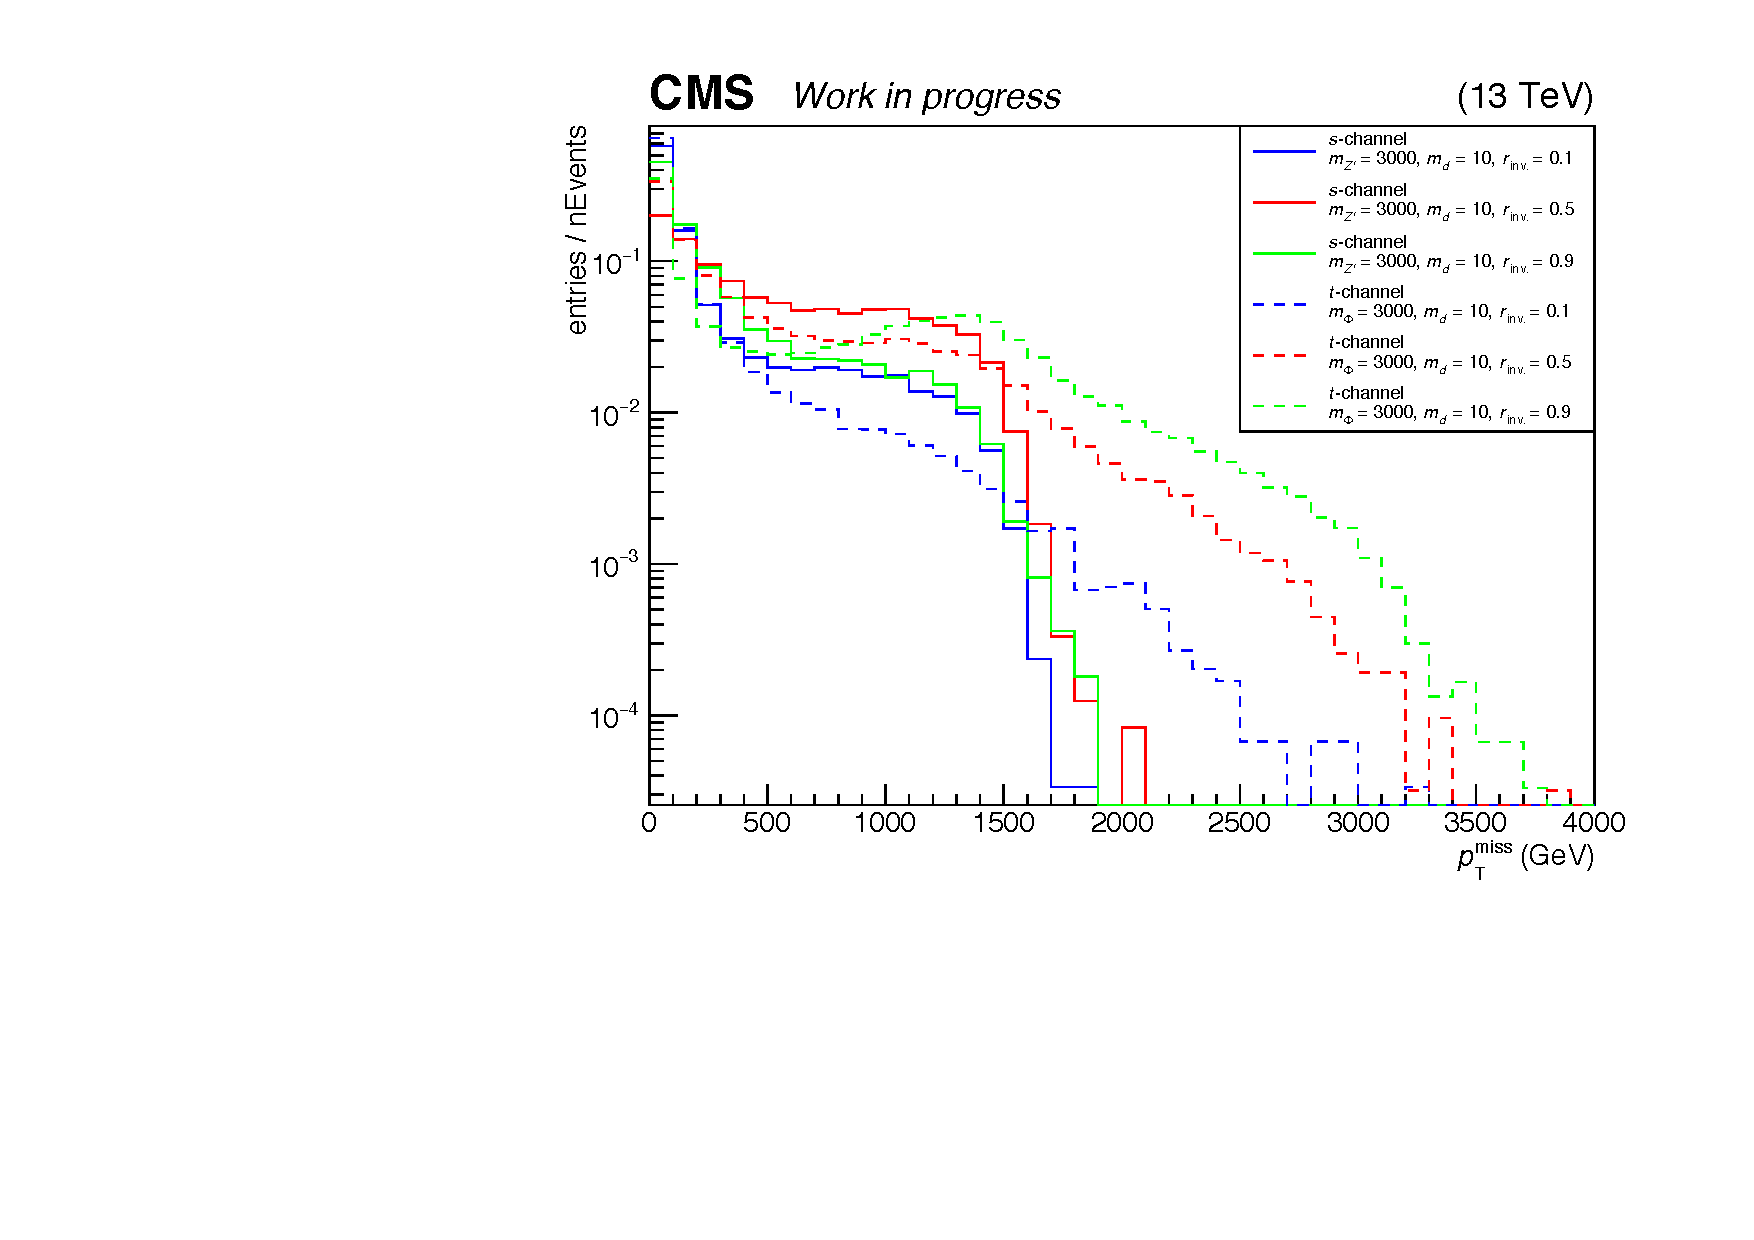
\includegraphics[width=0.75\textwidth]{./sec35/AEPSHEP/MET.pdf}
\caption{The \ptmiss\ spectrum for the $s$-channel (solid lines) and $t$-channel (dashed lines) semi-visible jet models. All parameters are kept the same except \rinv, which is varied to demonstrate its effect on the kinematics.}
\end{figure}

\begin{figure}[H]
\centering
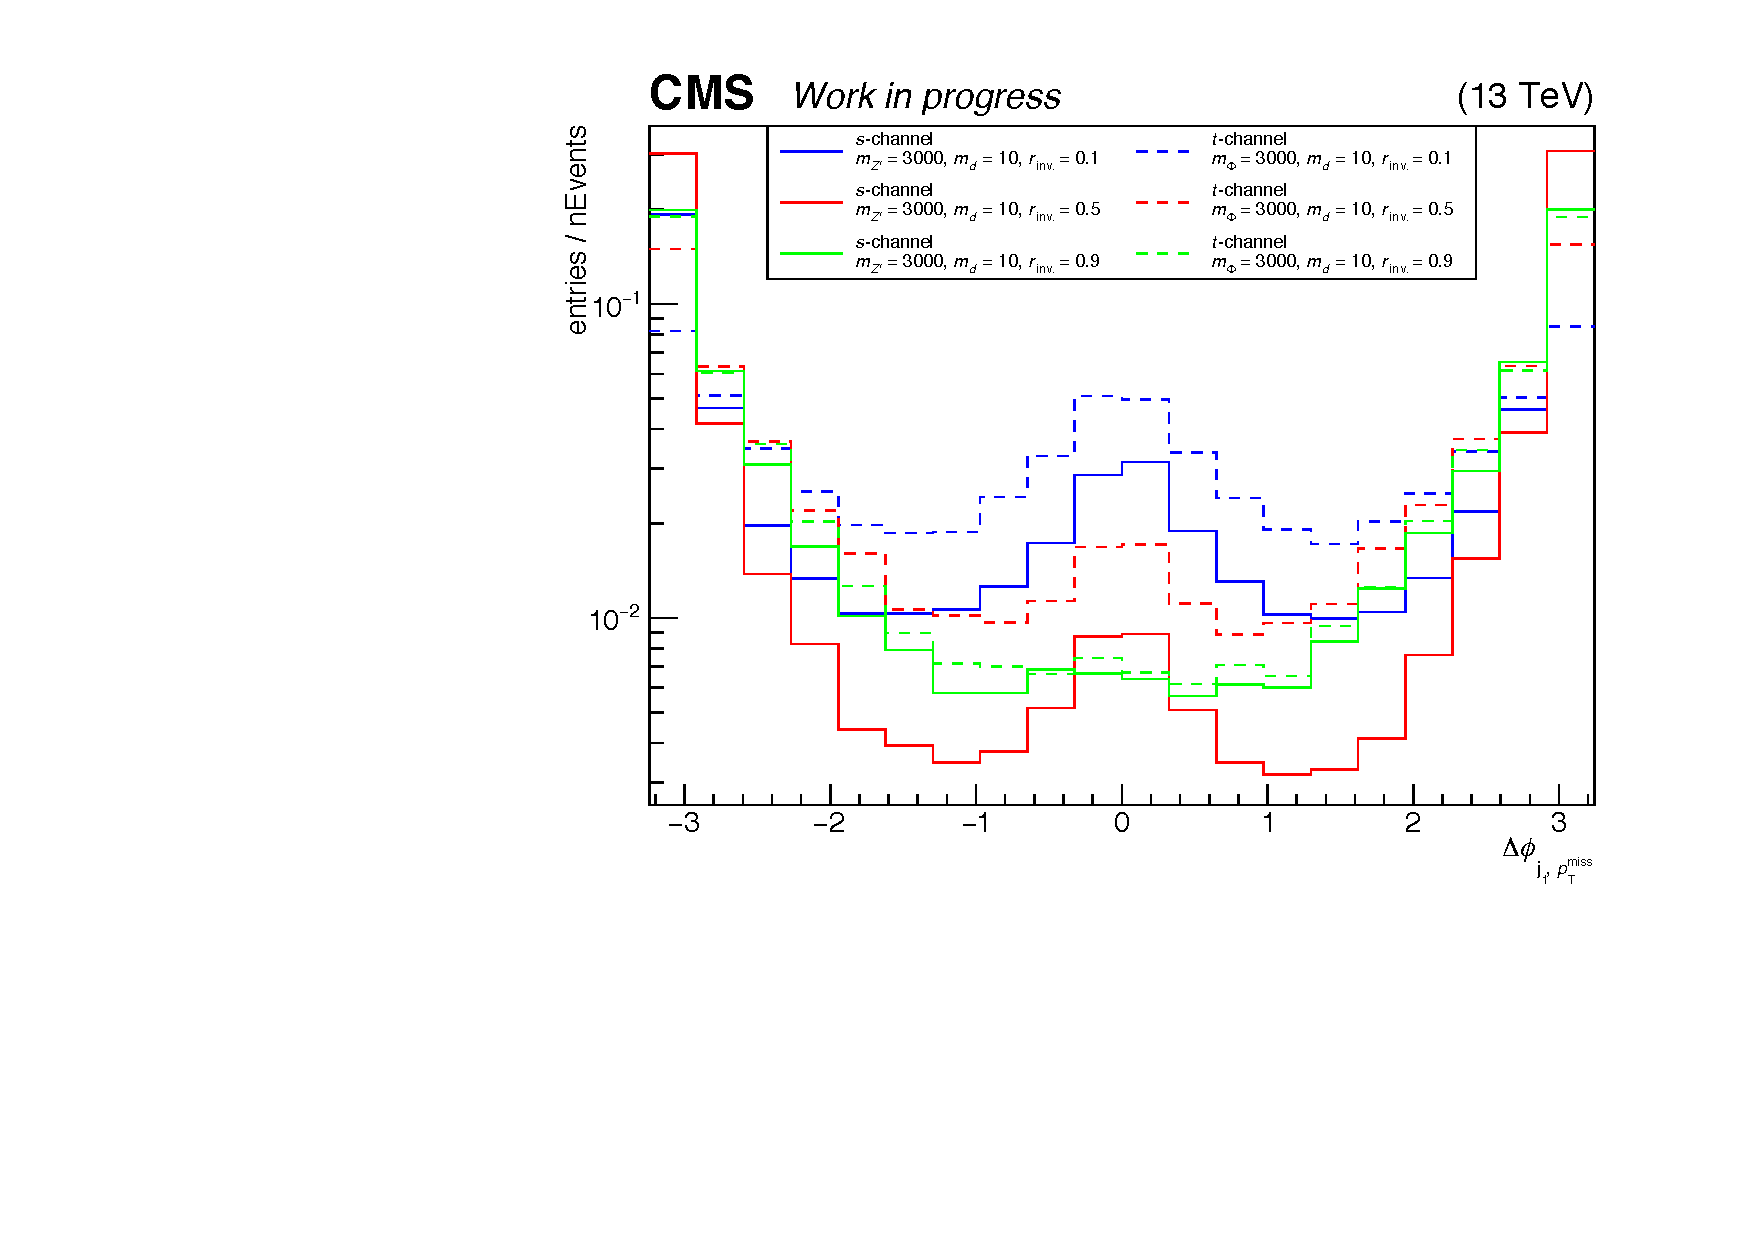
\includegraphics[width=0.75\textwidth]{./sec35/AEPSHEP/dPhiMetJ.pdf}
\caption{$\Delta\phi$ between the \ptmiss\ and the leading jet for the $s$-channel (solid lines) and $t$-channel (dashed lines) semi-visible jet models. All parameters are kept the same except \rinv, which is varied to demonstrate its effect on the kinematics.}
\end{figure}

In the first plot, as expected, the $s$- and $t$-channel distributions look very different. For the $t$-channel, \rinv\ parameter affects the distributions as it should. A higher value yields more dark particles, and so more MET. The $s$-channel curves are less affected, however there is a sharp decline at roughly $m_{Z'}/2$. This is due to the nature of the portal. There's a resonant production of the $Z'$, that decays into typically 2 jets. These should be symmetric in initial \pT\ and be produced back-to-back. So the maximum \pT\ of a SVJ (and therefore MET if all the particles remain invisible) will be $m_{Z'}/2$, hence the sharp decline afterward. If both jets have an invisible component (even if the total "dark" \pT\ is $> m_{Z'}/2$), the MET will be lower because it's formed from a \emph{vector} sum. As the $t$-channel process is not a resonance and is just an exchange of the $\Phi$ mediator, its mass is less directly important. The jet \pT\ (and therefore MET) is not limited by the mass of the mediator. This is exhibited in the plot where there are events with \ptmiss\ $>$ $m_{\Phi}$. While there are slight peaks in the $t$-channel curves for \rinv\ $= 0.5, 0.9$ close to $m_{\Phi}/2$, we haven't figured out why, quite yet.

The second plot also shows what we expect. Having dijet events most of the time allows us to split this plot into three cases. Case 1 is where the MET is aligned with the leading jet, yielding $\Delta\phi \sim 0$. Case 2 is when the leading jet recoils from the MET (if say, the second jet retains a high invisible fraction), so $\Delta\phi \sim \pi$. Case 3 is everything else: each jet contains an invisible component (which may not be antipodal) and so the resultant MET points somewhere between the two jets.

After the conference, I also presented on SVJ for the Bristol student seminar: \href{run:./sec35/20181030 Dark Matter Searches at CMS at 13 TeV.pdf}{20181030 Dark Matter Searches at CMS at 13 TeV.pdf}.

We have an analysis note on GitLab: \url{https://gitlab.cern.ch/tdr/notes/AN-19-061}, with some general instructions on working with it(\url{https://twiki.cern.ch/twiki/bin/viewauth/CMS/Internal/TdrProcessing}).

% -------- OTHER STUFF -------- 
$N$-subjettiness approach to identifying subjets:~\cite{Thaler:2010tr}.
More on jet substructure:~\cite{Freytsis:2014hpa}.
Running quark masses:~\cite{Bednyakov:2016onn}.
Comprehensive paper on various DM MET+X searches:~\cite{Aaboud:2019yqu}.
% --------------------------------------
